% !TEX program = xelatex
% 編譯指令：xelatex 專題簡介.tex
\documentclass[12pt]{article}

\usepackage{xeCJK}
\usepackage{geometry}
\usepackage{graphicx}
\usepackage{amsmath}
\usepackage{enumitem}
\usepackage{ragged2e}

% ---- 版面（收緊以容納 2 頁）----
\geometry{a4paper, top=1.6cm, bottom=1.5cm, left=2.2cm, right=2.2cm}
\setlength{\parindent}{0pt}
\setlength{\parskip}{3pt}
\linespread{1.15}

% ---- 中文字型：楷體（標楷體 風格）----
\setCJKmainfont[AutoFakeBold=2.2, AutoFakeSlant=0.15]{AR PL UKai TW}

% ---- 英數字型：襯線（Times 風格）----
\setmainfont{Latin Modern Roman}

% ---- 條列符號：● 實心 ----
\setlist[itemize,1]{label=$\bullet$, leftmargin=1.8em, itemsep=2pt, topsep=2pt}

\begin{document}

% ======== 標題區 ========
\begin{center}
  {\bfseries\fontsize{20pt}{24pt}\selectfont
    全域運動補償之指向性多目標追蹤}\\[8pt]
  {\fontsize{15pt}{19pt}\selectfont
    Referring Multi-Object Tracking aided by\\[2pt]
    Global Motion Compensation}
\end{center}

\vspace{4pt}

% ---- 右對齊資訊欄 ----
\begin{flushright}
  \begin{minipage}{0.62\textwidth}
    \begin{flushleft}
      指導教授：朱威達 \\[2pt]
      專題成員：白昕宸、王駿愷、彭以呈 \\[2pt]
      開發工具：Python、PyTorch、OpenCV\\[2pt]
      測試環境：Ubuntu 22.04、Refer-KITTI 資料集
    \end{flushleft}
  \end{minipage}
\end{flushright}

\vspace{4pt}

% ======== 一、簡介 ========
{\bfseries\fontsize{15pt}{19pt}\selectfont 一、簡介}
\vspace{2pt}

\justifying
在車載攝影機拍攝的影片中，畫面中物體的位移不一定代表物體本身正在移動，也可能源自攝影機的前進、轉向或晃動。如何區分物體的真實運動與相機自我運動（ego-motion），是動態場景理解與目標追蹤的核心問題；若無法有效分離兩者，系統便容易誤判物體的運動狀態，連帶影響追蹤與辨識結果。

此問題在\textbf{指向性多目標追蹤（Referring Multi-Object Tracking, RMOT）}中尤為明顯。RMOT 須在輸入影片與自然語言描述（如 \textit{moving cars}、\textit{turning vehicles}）後，從眾多追蹤目標中找出符合描述者；然而現有方法或仰賴視覺外觀特徵，或僅以原始邊界框位移作為運動線索，皆未補償相機的自我運動；當畫面位移混雜物體運動與相機運動時，模型便難以正確判斷涉及運動語意的描述。

為此，本研究提出 \textbf{GMC-Link}：透過\textbf{全域運動補償（Global Motion Compensation, GMC）}預估相機運動，萃取物體的真實殘餘運動資訊，與語言特徵對齊後，融合至既有 RMOT 模型輸出，藉以強化對運動語意描述的辨識能力。

\begin{itemize}
  \item \textbf{全域運動補償（GMC）}：以 ORB 特徵點搭配 BFMatcher（Hamming + Lowe's ratio 0.7）比對，經 RANSAC 估計\textbf{單應性矩陣（homography）}建立相鄰影格間的背景對映，並以前景遮罩避免誤抓物件特徵，確保補償的是相機而非物體運動。
  \item \textbf{累積單應性與多尺度殘餘速度}：保存物件\emph{原始未變形}中心座標，以累積複合單應性一次性校正，計算\textbf{三個時間尺度（gap = 2, 5, 10 影格）}的殘餘速度（原始速度 $-$ 相機速度），輸出含多尺度位移、寬高變化、中心座標、尺寸與訊噪比的\textbf{13 維運動向量}。
  \item \textbf{運動--語言對齊}：採\textbf{共享權重（shared-weight）}雙塔架構，運動 13D 與語言 384D 各經 Linear adapter 投影至 256D，再通過共享 MLP 主幹並 L2 正規化；以對稱式 InfoNCE Loss 訓練，推論時直接輸出原始\textbf{餘弦相似度（cosine similarity）}。
  \item \textbf{決策層線性加成融合}：以 $\text{final} = \text{model\_logit} + \alpha \cdot (sc \cdot \text{raw\_cos} + thr)$ 將 GMC 運動分數加成至原模型輸出，依運動／外觀兩軸分別校準後送入 HOTA 評估，判定是否匹配。
\end{itemize}

語言端以 SentenceTransformer（all-MiniLM-L6-v2，384D）編碼描述句。整體系統架構如圖一所示。

\begin{center}
  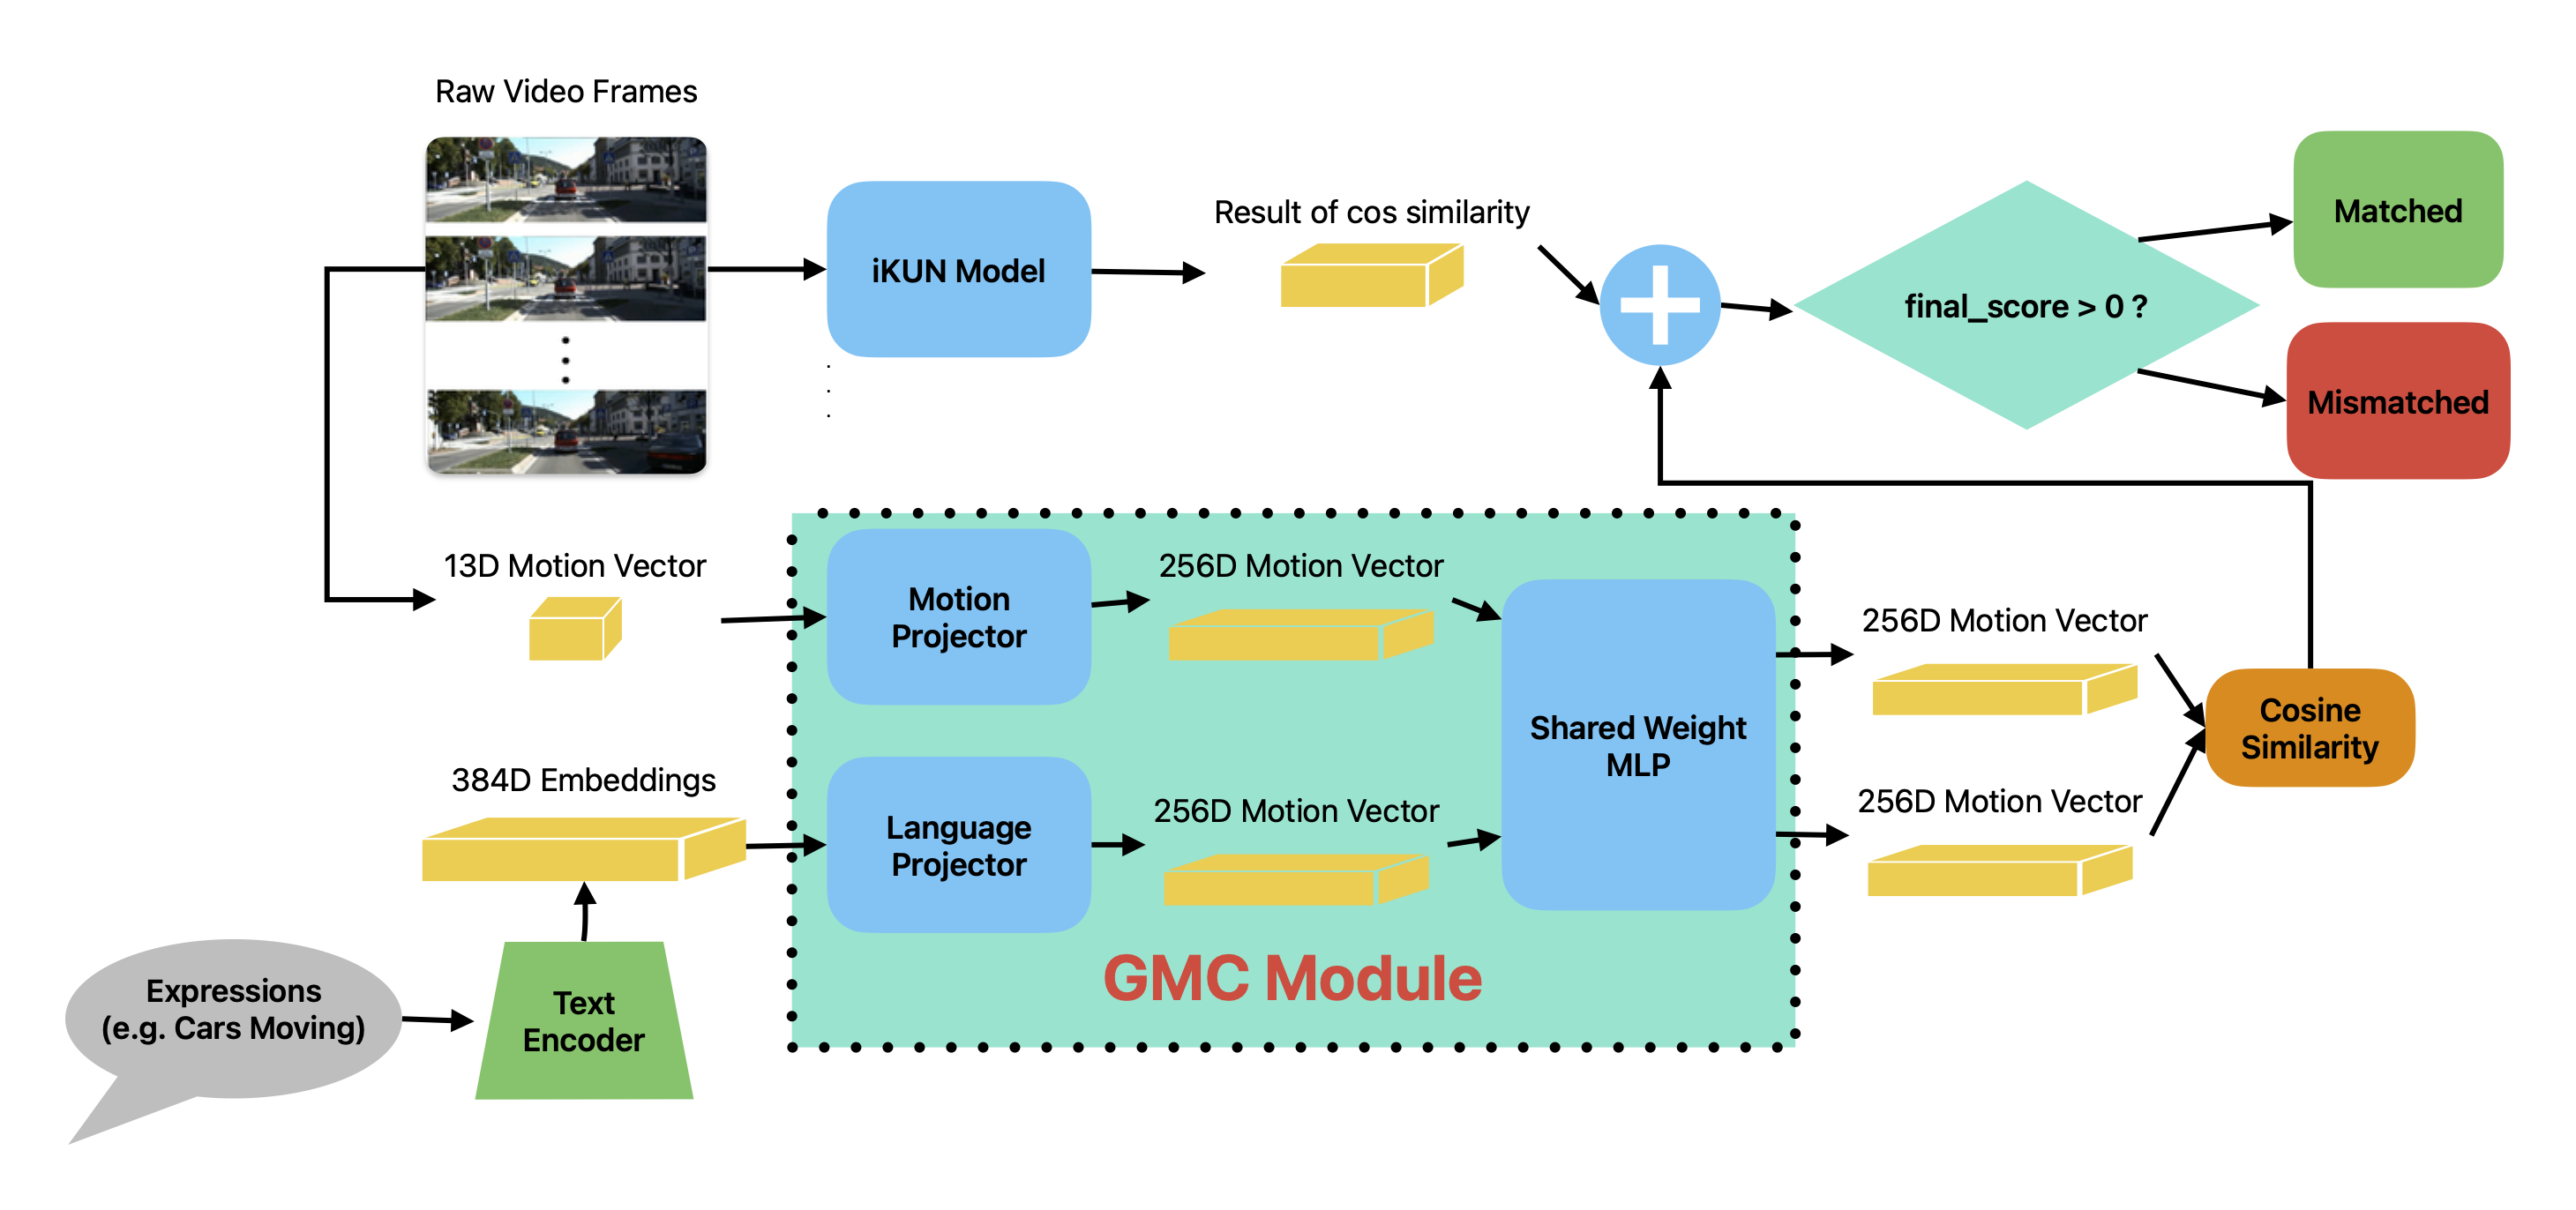
\includegraphics[width=0.72\textwidth]{framework_new.png}\\[2pt]
  {\small（圖一）GMC-Link 系統架構圖}
\end{center}

% ======== 二、測試結果 ========
{\bfseries\fontsize{15pt}{19pt}\selectfont 二、測試結果}
\vspace{2pt}

\justifying
本研究於 \textbf{Refer-KITTI} 資料集上，對\textbf{三種基礎追蹤架構}進行交叉驗證，採 \textbf{$n=3$ 多隨機種子}、以 \textbf{pooled HOTA} 為指標評估融合前後表現。由表一可見，GMC-Link 在 \textbf{3 個架構中有 2 個超越原論文}，且增益穩定：

\begin{center}
  \small
  \begin{tabular}{l c c c c}
    \hline
    架構 · 資料集      & 原模型    & + GMC-Link      & 原論文    & 較原論文            \\
    \hline
    iKUN · V1     & 44.224 & \textbf{44.634} & 44.564 & \textbf{+0.070} \\
    FlexHook · V1 & 53.110 & \textbf{53.526} & 53.824 & \textbf{-0.298} \\
    FlexHook · V2 & 42.526 & \textbf{42.807} & 42.526 & \textbf{+0.281} \\
    \hline
  \end{tabular}\\[3pt]
  {\small （表一）融合前後 pooled HOTA 比較。}
\end{center}

GMC-Link 的增益\textbf{主要來自運動類別描述}（如「moving cars」「turning vehicles」）——這正是純外觀模型最弱、也是本系統設計初衷所在。以 iKUN · V1 為例，原模型於運動描述上 HOTA 僅 \textbf{25.531}，遠低於靜止描述的 43.914，落差近 \textbf{18 分}；加入 GMC-Link 後提升至 \textbf{30.093（+4.562）}，大幅彌平此落差。三種架構在運動描述上皆獲提升（見表二）：

\begin{center}
  \small
  \begin{tabular}{l c c c}
    \hline
    架構 · 資料集      & 原模型    & + GMC-Link & 增益              \\
    \hline
    iKUN · V1     & 25.531 & 30.093  & \textbf{+4.562} \\
    FlexHook · V1 & 43.981 & 45.785  & +1.804          \\
    FlexHook · V2 & 48.018 & 48.758  & +0.740          \\
    \hline
  \end{tabular}\\[3pt]
  {\small （表二）僅運動類別描述之 pooled HOTA 增益。}
\end{center}

此結果印證\textbf{全域運動補償為運動語意判斷的關鍵}：相較直接採用原始邊界框位移的方法，ORB 加單應性的幾何補償能有效分離相機運動，是運動類別描述能否正確匹配的決定性元件。進一步分析顯示，\textbf{多尺度時序速度}（同時捕捉短／中／長期運動模式）為對齊分離度貢獻最大的單一設計；\textbf{訊噪比特徵}雖未提升平均分離度，卻顯著降低了預測變異。

整體而言，本系統以\textbf{決策層加成}方式接入，不更動亦不重訓基礎模型，可泛化至多種對空間運動不敏感（spatially-ignorant）的視覺--語言追蹤框架；並透過\textbf{逐類別 GMC 關聯性調節}（運動軸與外觀軸採不同校準尺度），抑制運動訊號於純外觀描述（如「black cars」）上的雜訊干擾，達成從感知、對齊、融合到判定的完整增強流程。

\end{document}
